\documentclass[english]{thesis}
\usepackage[cpp]{mypackage}

\title{Project 1}
\school{School of Data and Computer Science}
\author{Hongzheng Chen}
\stunum{17341015}
\headercontext{Parallel and Distributed Computing}

\begin{document}

\maketitle

\section{Problem Description}
Implement a multi-access threaded queue with multiple threads inserting and multiple threads extracting from the queue. Use mutex-locks to synchronize access to the queue. Document the time for 1000 insertions and 1000 extractions each by 64 insertions threads (Producers) and 64 extraction threads (Consumer).

\section{Solution}
To enable portable cross-platform programming, the native support of multithreading has introduced to C++11.
Thus, I use the facility of multithreading in C++11, which makes the program more stable and thread-safe.

Two functions named \verb'Producer' and \verb'Consumer' are implemented in the program.

The \verb'Producer' takes in the value and push it into the queue, while the \verb'Consumer' pop the front value out of the queue.
If the length of the queue is less than 1000, the \verb'Producer' consistently pushes a new value into the queue.
And if the queue is not empty, the \verb'Consumer' continuously pops the values from the queue.

To avoid conflicts, two mutex-locks \verb'push_mutex' and \verb'pop_mutex' are defined as global variables.
When the \verb'Producer' and \verb'Consumer' begin to function, these two locks are respectively added to them.
In this way, only one thread is able to access the queue at a time.
C++11 uses \verb'lock_guard<mutex>' to safely manage the locks.
The locks will only function in their scopes.
After the scopes, they will be automatically destroyed.

To make the program flexible, I use templates for \verb'Producer' and \verb'Consumer', which enable different types of queues.

Moreover, I implement the single thread queue baseline for comparison.
\verb'Makefile' is written for the project.
Type \verb'make' to do the compilation and type \verb'make run' to run the experiment.

The machine used in this experiment has Intel Core i7-7700HQ processors (8 cores) running at 2.80GHz with Ubuntu 18.04 LTS.
The program is compiled by \verb'gcc' (v7.3.0) with \verb'-std=c++11' and \verb'-pthread'.

\section{Experimental Results}
The experimental results are shown in Fig.~\ref{fig:result}.
The experiment is run for several times.
\begin{figure}[H]
\centering
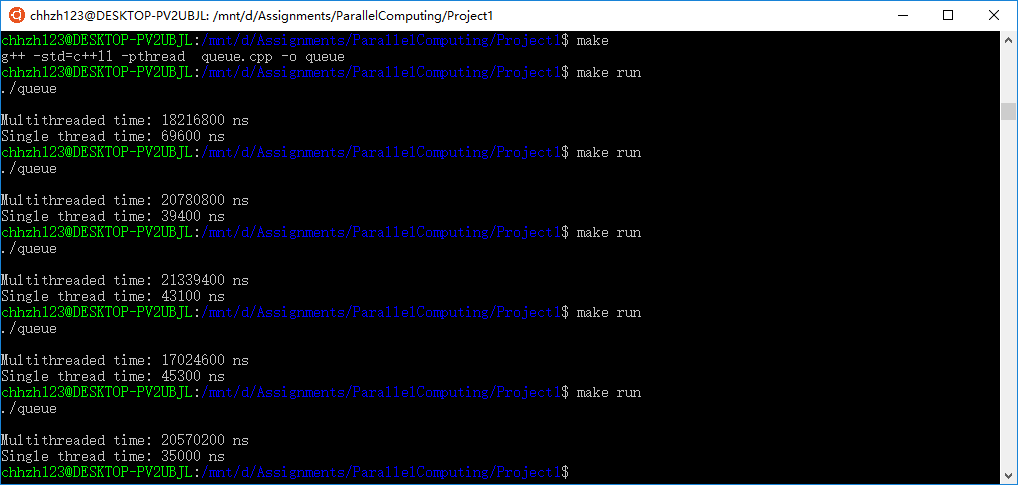
\includegraphics[width=0.8\linewidth]{results.PNG}
\caption{Running time of single-threaded and multi-threaded queue}
\label{fig:result}
\end{figure}

We can clearly see that the single-threaded queue is much faster than the multi-threaded queue, which is due to the great overhead of creating several threads and the so small-scale data.
Moreover, since 64 threads functions on only one value and one queue, there exists lots of conflicts, which also hampers the performance.

To make multi-thread queue truly function, more workload should be added to each thread, or more queues are considered.

\appendix
\appendixconfig
\section{Programs}
The outputs have been deleted for exact timing.
Define the \verb'DEBUG' variable may enable the outputs.
\begin{lstlisting}
#include <iostream>
#include <thread>
#include <mutex>
#include <queue>
#include <chrono> // timing
using namespace std;

using Clock = chrono::high_resolution_clock;

#define MAX_THREAD 64
#define MAX_NUM 1000

mutex push_mutex;
mutex pop_mutex;

template <class T>
void Producer(queue<T>& q, T& val)
{
	while (1){
		lock_guard<mutex> guard(push_mutex);
		if (val < MAX_NUM){
			q.push(val);
			val++;
		} else
			break;
	}
}

template <class T>
void Consumer(queue<T>& q)
{
	while (1){
		lock_guard<mutex> guard(pop_mutex);
		if (!q.empty()){
#ifdef DEBUG
			cout << q.front() << " ";
#endif
			q.pop();
		} else
			break;
	}
}

int main()
{
	queue<int> q;
	thread t[MAX_THREAD];
	int cnt = 0;

	auto t1 = Clock::now();

	for (int i = 0; i < MAX_THREAD; ++i)
		t[i] = thread(Producer<int>,ref(q),ref(cnt));
	for (int i = 0; i < MAX_THREAD; ++i)
		t[i].join();

	for (int i = 0; i < MAX_THREAD; ++i)
		t[i] = thread(Consumer<int>,ref(q));
	for (int i = 0; i < MAX_THREAD; ++i)
		t[i].join();
	cout << endl;

	auto t2 = Clock::now();
	cout << "Multithreaded time: " << chrono::duration_cast<chrono::nanoseconds>(t2 - t1).count() << " ns" << endl;

	t1 = Clock::now();
	for (int i = 0; i < MAX_NUM; ++i)
		q.push(i);
	for (int i = 0; i < MAX_NUM; ++i)
		if (!q.empty()){
#ifdef DEBUG
			cout << q.front() << " ";
#endif
			q.pop();
		}
	t2 = Clock::now();
	cout << "Single thread time: " << chrono::duration_cast<chrono::nanoseconds>(t2 - t1).count() << " ns" << endl;
	
	return 0;
}
\end{lstlisting}

\end{document}

% problem description, solution, experimental results, problems when implementation